\subsection{Feedback loops}

When there is a lack of feedback from customers/users, then someone has to decide.


when there are multiple competing objectives among different stakeholders in a zero sum use of resources, how to determine what's best? Typically there are feedback loops to guide progress. When feedback loops are weak or not present, then the most powerful stakeholder (which is distinct from the biggest or loudest) will dominate. 

Example of no feedback loop:
when there is a benefit to a small group and the cost is to a larger group



Suppose I earn \$100,000 and the tax rate is 30\%. Then my tax money sent to the government is \$30,000.

"In 2021, the [US] government collected \$4.05 trillion in revenue."
\footnote{source: Government Revenue | U.S. Treasury Data Lab}

My taxes of \$30,000 is
30000/4050000000000 = 0.00000074\%

When I do not maximize the effectiveness of \$1,000,000 of government money, of that misallocated money \$0.0074, or about one penny, was taxes I paid. The feedback loop is weak.

Federal pay is limited to about \$220,000\footnote{https://en.wikipedia.org/wiki/Executive\_Schedule}, so that raises the feedback to 2 pennies.

The lack of feedback allows waste to go unfelt. There's no immediate consequence.
Waste is indistinguishable from not enough funding or insufficient skills 




Feedback loop:
\begin{center}
\begin{figure}[ht]
    \centering
    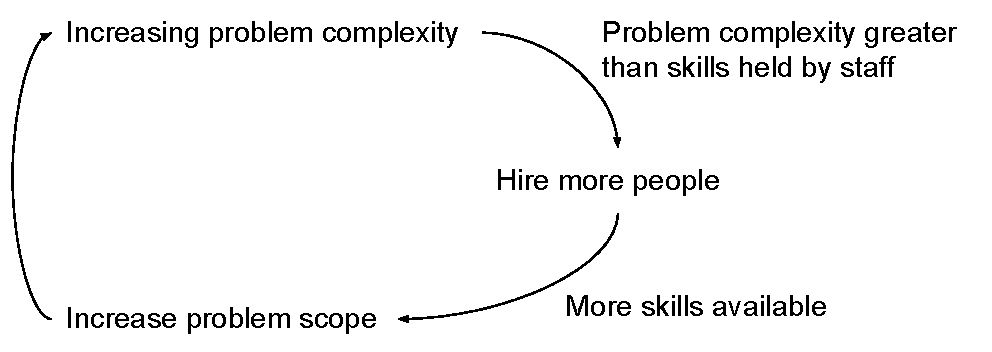
\includegraphics[width=0.8\textwidth]{images/feedback_loop_complexity_and_staffing}
    \caption{Complexity requires more staffing; having more staff means more skills are available; under-utilized staff skills make room for more scope; more scope adds to complexity.}
    \label{fig:complexity_and_staff_growth}
\end{figure}
\end{center}
